\section{Data with Dissimilar Appearances}
\label{sec:changing_environment}	

	\begin{figure}[t]
	\centering
    \begin{minipage}{0.44\linewidth}
    		\centering
   			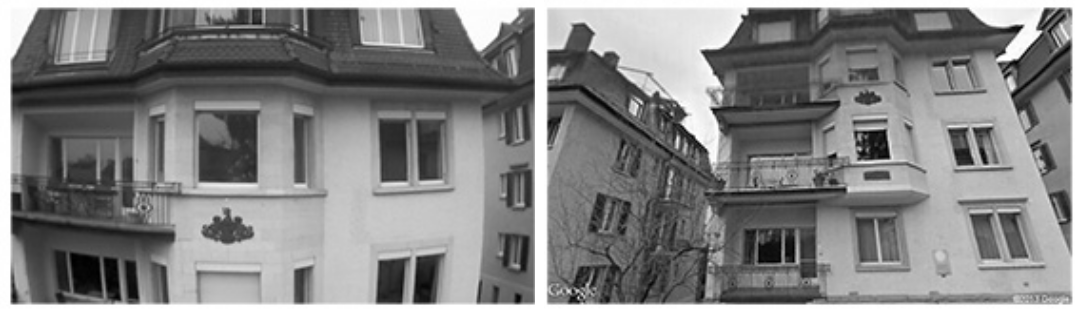
\includegraphics[width=\linewidth]{changes/viewpoint.png}

			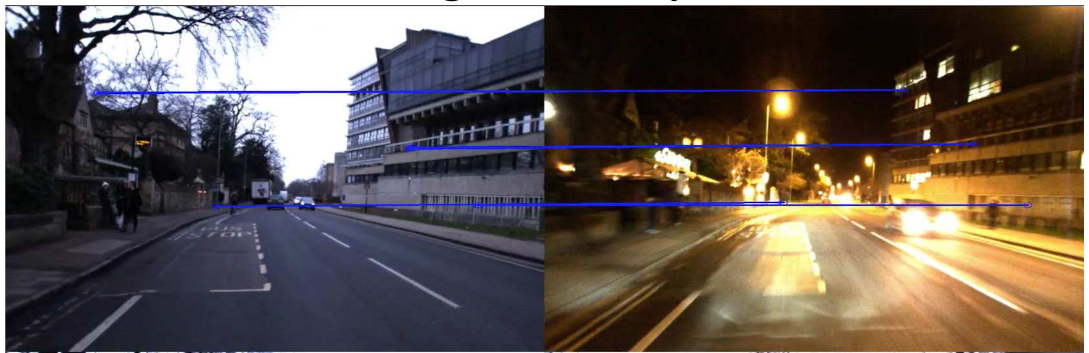
\includegraphics[width=\linewidth]{changes/daynight2.png}
			
			\subfigure[][Appearance changes]{\label{fig:changes}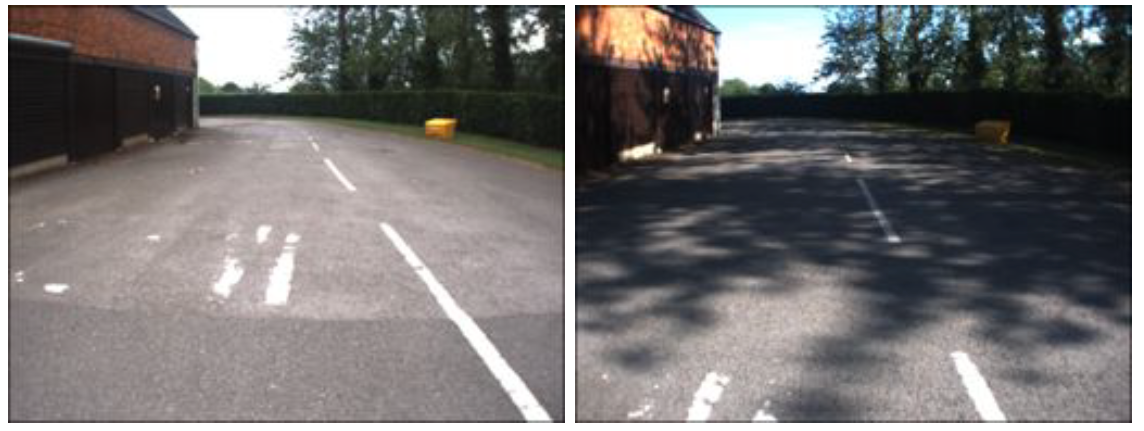
\includegraphics[width=\linewidth]{changes/shadow.png}}
    \end{minipage}
	\hfill
	\begin{minipage}{0.53\linewidth}
   		\subfigure[][Cross-view]{\label{fig:cross-view}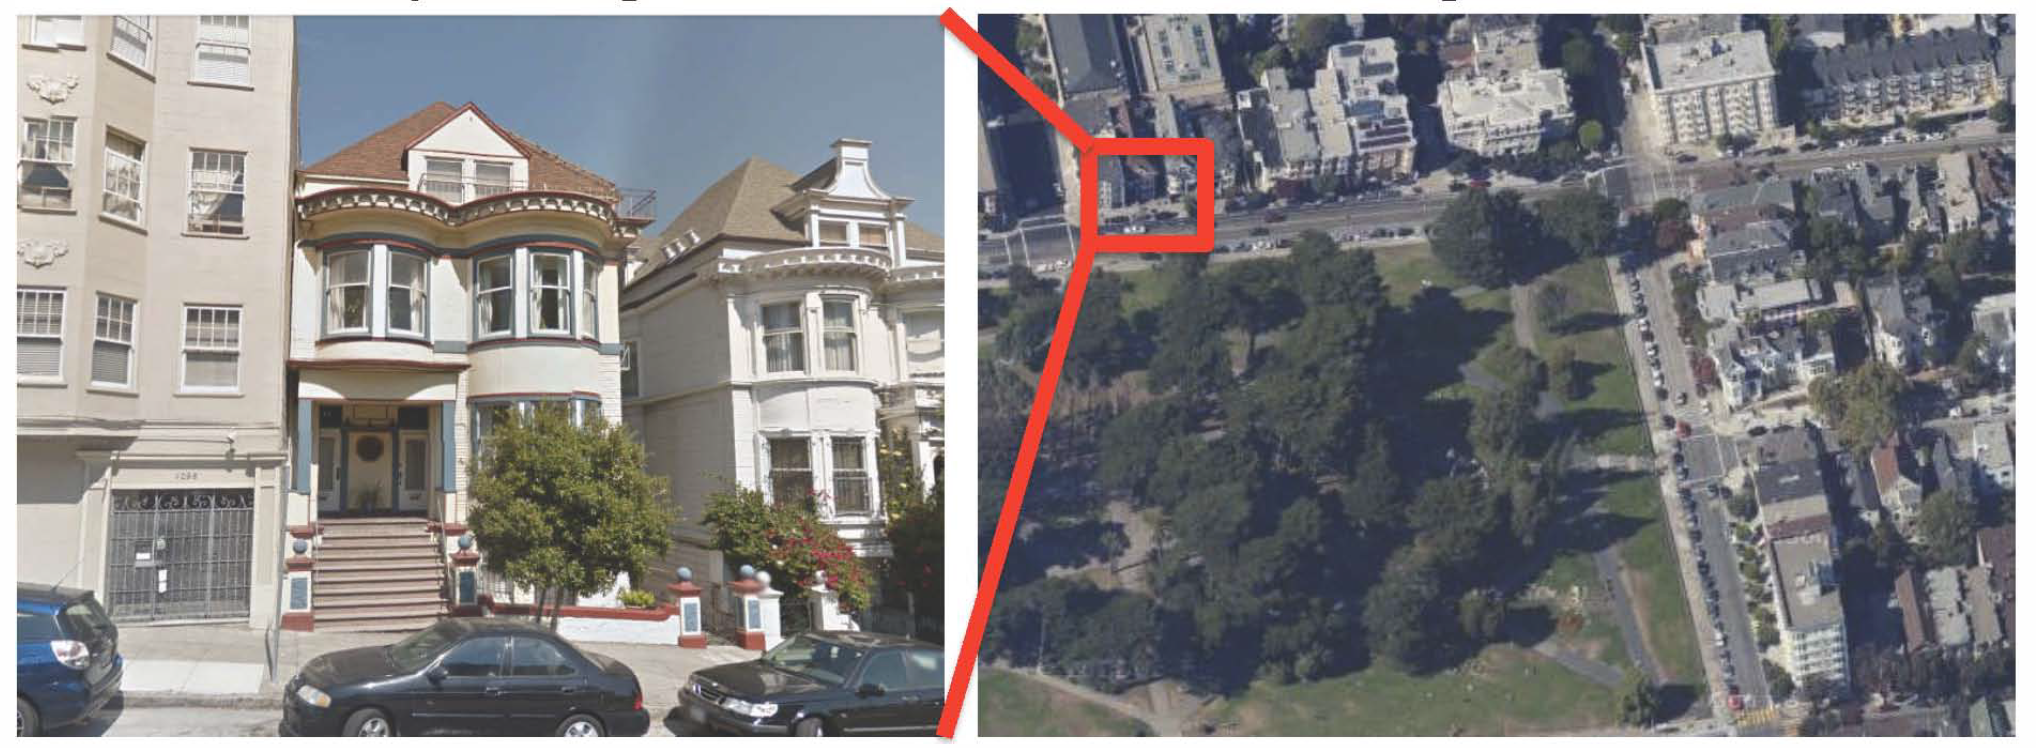
\includegraphics[width=\linewidth]{changes/cross-view.png}}
   		    
   		\subfigure[][Cross-domain]{\label{fig:cross-domain}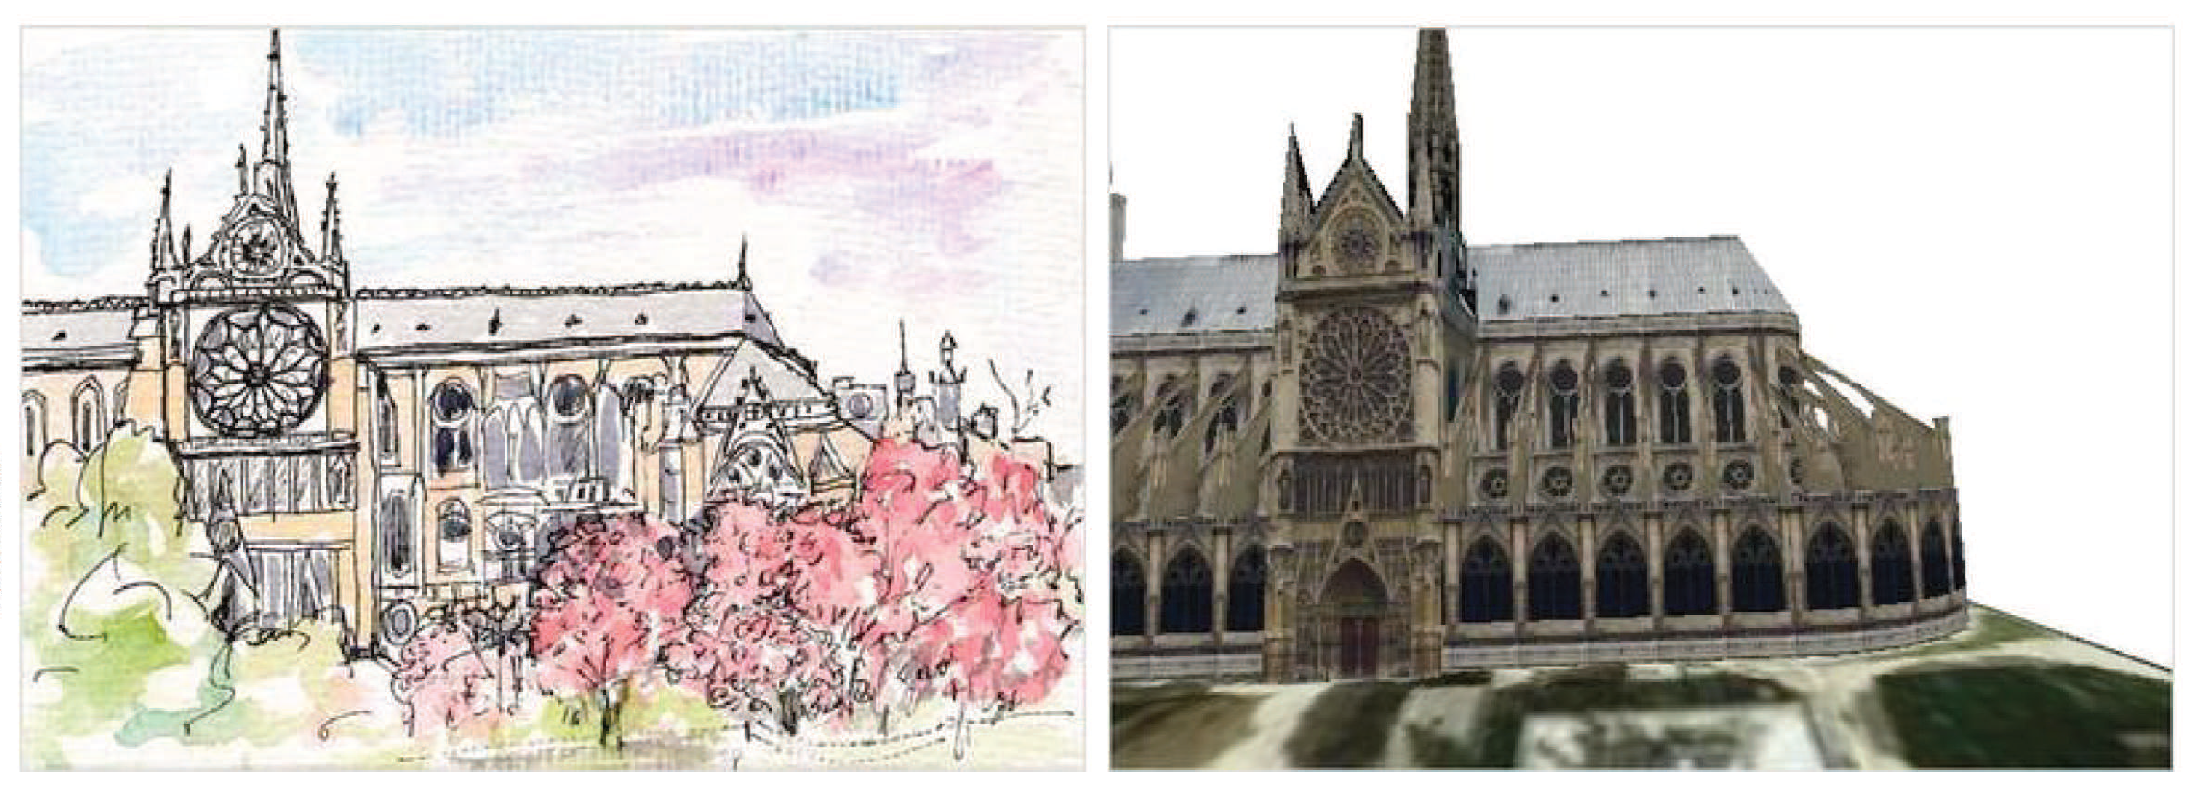
\includegraphics[width=\linewidth]{changes/cross-domain.png}}
	\end{minipage}
	\caption[Illustration of appearance changes present in \acs*{vbl} system]{\textbf{Illustration of appearance changes present in \ac{vbl} system:} \ref{fig:changes}~Visual dissimilarity between the query (left) and the closest image in the database (right). Cause of the change, from top to bottom:~viewpoint differences~\citep{Majdik2013}, daytime to nighttime image matching~\citep{Porav2018} and shadow interferences from~\citep{Corke2013}. \ref{fig:cross-view}~Cross-view localization system~\citep{Lin2015}:~left represent the ground-level query image and right the bird's eye view of the same scene. \ref{fig:cross-domain}~Cross-domain \ac{vbl} system~\citep{Aubry2014}:~on the left the query painting and on the right the corresponding pose according to a 3D model. \label{fig:data_changes}}
\end{figure}


	As pointed out by \citet{Lowry2016}, permanent changes occurring in our environment is a huge concern in vision domain. In \ac{vbl}, to the difference of SLAM based navigation methods \citep{Garcia-Fidalgo2015,Lowry2016}, the environment representation (i.e. the database) is most of the time acquired at a single date and query can be opposed to the system years after. To take into account local changes of the environment the database needs to be updated. Depending on the size of the covered area, database update can be a costly operation. Thus, an ideal \ac{vbl} system should be able to handle minor visual changes from various sources: daily and season cycle, difference in viewpoint or modifications of the local geometry of the scene. In this section we review selected \ac{vbl} papers that tackle the problem of visual changes in the environment. We dedicate the second part of the section to localization methods that consider extreme appearance changes between the query and the database, namely: cross-view and cross-domain \ac{vbl} systems.
	
	\subsection{Appearance changes}
	\label{subsec:appearance}
		\paragraph{Viewpoint changes.}
			\label{para:viewpoint}
			Common visual acquisition systems capture a part of the environment lying inside the frustum of the sensor. Indeed, perspective camera are oriented-device and due to the complex geometry of our surrounding environment, viewpoint changes in visual data can impact drastically the appearance of a scene. Visual disturbance induced by viewpoint changes is illustrated in figure~\ref{fig:changes}, top images. To handle those changes, local descriptors described in \S\ref{subsec:local_feature} have been widely used. By describing partial areas of the whole scene, local features are naturally robust to a certain amount of changes introduced by difference in viewpoint and occlusion. \citet{Wan2014} treat extreme viewpoints changing (when the camera are facing each other) in repetitive lunar environment. To achieve \ac{vbl} in such conditions they match the ground part of the image (which is subject to large affine distortion) with a fully affine invariant feature~\citep{Morel2009}. In~\citep{Garg2018a}, authors use semantically weighted keypoints to match images taken with opposite viewpoints.
			
			Image rectification~\citep{Forstner2016} is also employed in \ac{vbl} to minimize appearance changes introduced by different viewpoints. With strong assumption on the environment where the localization is performed (\textit{e.g.} such as Manhattan world assumption~\citep{Murillo2013,Cham2010}), images rectification ensure that facing direction of all visual data will be barely the same. With the hypothesis of an urban scene, vanishing points can be extracted~\citep{Lezama2014,Hartley2003,Forstner2016} and images rectified to display front facing buildings~\citep{Robertson2004,Chen2011,Morago2016,Arth2015,Cham2010}.
			
			Other approaches consists of filling the database with additional data to cover all the possible viewpoints for a given environment. \citet{Milford2015} generate translated view on a database road-circuit for preventing miss-matches if the car, carrying the acquisition system, is moving on a different traffic way than the one used to collect the database. Notice the use of a depth from monocular images \ac{dl} model to produce synthetic shifted-views. Work from~\citep{Irschara2009,Aubry2014,Torii2015} increase the number of documents in the database by automatic data generation to ensure that whatever the viewpoint of an incoming query, a document displaying a similar view can be retrieved. \citet{Majdik2013} perform air-ground matching of picture taken by a Micro Air Vehicle (MAV) against street view images. The main challenge outlined in this paper is the large difference in angle viewpoint. Authors generate artificial view from both the database and the query image to handle the affine transformation introduced by altitude differences (inspired by the work of~\citep{Morel2009}). Inloc~\citep{Taira2018,Taira2019} introduces dense pose verification with view synthesis for indoor localization: artificial viewpoints are rendered from a 3D model at putative query poses.
			
		\paragraph{Long-term localization.}
	       	\label{para:illum}
			As exposed in the introduction of this section, \ac{vbl} methods need to be robust to visual changes present in images taken at different times. These differences can be induced by: illumination changes across season, daily cycle, weather conditions, or dynamic changes in the scene (see figure~\ref{fig:changes} for illustration). \citet[Section VII]{Lowry2016} explore exhaustively Visual SLAM methods that perform strong illumination invariance place recognition (\textit{e.g.} SeqSLAM~\citep{Milford2012,Pepperell2014,Pepperell2016} or FAB-MAP~\citep{Cummins2008,Cummins2010,Paul2010}). In~\citep{Lowry2016a}, authors present an invariant-free image representation in order to overcome perturbation induced by long-term localization. \citet{Rosen2016} propose a model to take in account the features persistence, decreasing the probability of encountering a feature that have been met for the first time a long time ago. In the work of~\citet{Porav2018}, authors use \ac{gan} to produce time-shifted images before the localization task. For instance, they convert night-time images into daytime images to improve local feature matching across the query and references data. This method can also be used for inter-season localization. \citet{Bescos2019} handle explicitly non-sustainable visual elements, such as car or pedestrian, in order to create invariant image representation. They detect disruptive objects in images, remove it and finally inpaint the modified element thanks to a \ac{gan} trained on synthetic data. In~\citep{Naseer2017a}, a adaptive learned mask is applied on the input images. This mask aims to remove non-persistent elements upstream of the image description.
			
			As mentioned previously, methods based on local descriptors are prompt to handle local changes in images due to dynamic modifications of the environment (\eg vegetation growing, buildings construction or annihilation, presence of pedestrians or vehicles, partial occlusions, etc.). Several investigations have been led for designing robust descriptors to local geometric changes. In~\citep{Kim2015,Linegar2016}, authors train SVM classifiers to discriminate strong and weak local features for the \ac{vbl} task. This method, and its continuation~\citep{Kim2017}, shows promising results where features are more often selected when they are attached to persistent objects, such as facades, and dismissed when they represent ephemeral or changing elements, such as people or trees. In general terms, pretrained network for semantic segmentation offer strong local description for long-term localization, as illustrated in~\citep{Mousavian2015,Garg2018a,Toft2018,Shi2019,Schonberger2017a}.
			
			In a more robotic-oriented-scenario, \citet{Muhlfellner2015} investigate map invariance representation when multiple instances of the same environment are available. On the other hand, learned descriptors show good performances if trained for the specific inter-season matching task~\citep{Carlevaris-Bianco2014}. \citet{Arandjelovic2017} train a \ac{cnn} for global description upon images from the Google Street View Time Machine to get diverse representation of the same scene captured over a period of ten years. From this kind of representation of the environment, persistent clues can be efficiently extracted~\citep{Neubert2015}. Similarly, \citet{kumar2017condition} proposes a CNN approach for place recognition across seasons. In~\citet{Germain2018}, authors use a \ac{cnn} as global descriptor for localization trained with explicit information about the outdoor condition of each example. Once trained, their descriptor can be used for cross-condition localization, as long as external conditions (\eg daytime, rain, etc.) are known at query time.
			
			In the following we report methods focusing on one specific problem induced by long-term localization. 

			\subparagraph{Dealing with Seasons \& Weather.}
				\citet{Valgren2010} have shown that usual local features, like SIFT or SURF, are not well suited for similarity association across season cycles. GRIEF local descriptor~\citep{Krajnik2017a} (derivatives of BRIEF~\citep{Calonder2010}) or ORB feature~\citep{Griffith2017} show better results for this task. Works described in~\citep{Krajnik2014,Krajnik2017a} model seasonal-like cycle in a probabilistic framework in order to downgrade features that are not likely to appear during a given period of time. A de-raining \ac{cnn} filter is proposed in~\citep{Porav2019} to improve localization with bad weather condition. Their model is trained with both synthetic and real data.
		
			\subparagraph{Dealing with Nocturnal illumination.}
				In some application, especially for vehicle localization, \ac{vbl} has to be performed during a complete day, including overnight~\citep{McManus2014,Milford2015} (see middle example of figure~\ref{fig:changes}). Dense descriptors'~extraction used in \citep{Torii2015} exhibit promising result for daytime to overnight images matching. At first glance, artificial lights ubiquitous in urban scene can be considered as sources of disruption. However, \citet{Nelson2015} focus on this particular clues to perform localization across only night road images. 
				
			\subparagraph{Dealing with Shadows.}
				Some researches focus on the specific perturbation introduced by shadow casting over images. \citet{Wan2016} outline that satellite and overhead images can change drastically in appearance depending on the relative position of the sun during the day. Authors show that Fourier transforms can be used to create shadow-invariant image representation. \citet{Corke2013} implement the shadow suppression method presented in~\citep{Finlayson2006} to localize street images with important depth artefacts projected by trees or buildings. This method still remains very sensor-dependent.

	\subsection{Cross-appearance localization}
	\label{subsec:cross_domain}
		Subsequent part focus on methods that reach an extreme with change-invariance consideration by creating cross-appearance algorithms for \ac{vbl}. We distinguish between two main categories of applications: cross-view \ac{vbl}, where authors localize a ground-view image against database of aerial images, and cross-domain \ac{vbl}, where the purpose is to localize images of various nature (like  ancient photographies, painting, sketching, etc.).
		
		\paragraph{Cross-view}
			\label{para:cross_view}
			Cross-view localization~\citep{Lin2013,Workman2015,Castaldo2015,Vo2016,Tian2017}, also denoted as ultra-wide baseline matching~\citep{Bansal2012}, consider the problem of ground level localization from aerial-level set of photo shoots (see figure~\ref{fig:cross-view} for an illustration of data association targeted by cross-view systems). Cross-view \ac{vbl} is motivated by the fact that satellite photographies are rich sources of information, available almost all over the globe. However, finding similarity between data acquired at a ground level and data captured with flying devices is a hard task due to the extreme change in viewpoint. In~\citep{Workman2015,Vo2016}, authors investigate the use of a CNN to automatically associate ground level images taken from street view service with fine-grained overhead images. \citet{Vo2016} compare several CNN architectures and conclude that triplet trained network provides the most suitable descriptors for cross-view matching. Rotation invariance between ground and overhead images is also studied through auxiliary loss and special training. Conditional \ac{gan} are explored in~\citep{Regmi2018} to generate ground level image from aerial footage (or vice versa). Authors show that the latent representation learned by the \ac{cnn} can be used as image feature for cross-view localization.
						
			In~\citep{Bansal2011,Bansal2012,Lin2015}, authors use bird's eye imagery to localize ground level snapshots. \citet{Bansal2011} method relies on ground level images rectification, like methods focused on viewpoint changes (refer to \S\ref{para:viewpoint}).
			
		\paragraph{Cross-domain}
			\label{para:cross_domain}
			Another field of research where the data association is very challenging is the cross-domain localization (an example of cross-domain \ac{vbl} is presented in figure~\ref{fig:cross-domain}). \citet{Russell2011} work, followed by \citet{Aubry2014} contribution, focus on the task of retrieving the pose of an old hand-drafted document (a sketch or a painting) according to a known realistic representation. In~\citep{Aubry2014}, hard training of HOG-based descriptors are used to capture the global shape of the architectural scene displayed in the documents, in the same manner as~\citep{Shrivastava2011}. Results are impressive, but the used descriptor is not robust to viewpoint changes. Cross-domain techniques are also used to recover the pose of ancient photographies and to confront them with current data \citep{Bae2010,Bhowmik2017}. \citet{Bhowmik2017} study a new approach for pairing various local descriptors in order to increase retrieval results depending on the targeted dataset. This method have been successfully applied to match ancient photographies and nowadays images.